\documentclass[a4paper,12pt]{article}
\usepackage[utf8]{inputenc}
\usepackage[french]{babel}
\usepackage[T1]{fontenc}
\usepackage[top=2cm,bottom=2cm,left=2cm,right=2cm]{geometry}
\usepackage{graphicx}
\usepackage{wrapfig}
\usepackage{url}

\begin{document}

\begin{titlepage}
	\begin{center}
		\Large{Année universitaire 2016-2017}\\
		\Large{Université de Caen Normandie}\\[1cm]
		
		\huge{Rapport sur la création de boutons dans l'interface graphique de l'IDE}\\
		\vspace{3cm}
		
		Emma MAUGER
		
	\normalsize{\textit{ ~ L2 Informatique}}\\
		\medskip
		\vspace{2cm}
				
	\end{center}
\end{titlepage}

\tableofcontents
\newpage

\section{Le bouton "Anlayse"}

\begin{figure}
	\begin{center}
		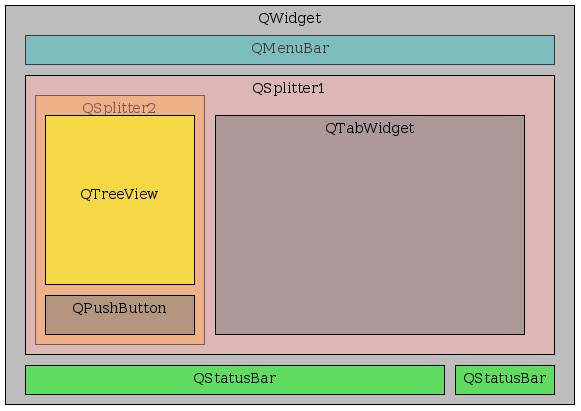
\includegraphics[scale=0.5]{images/ide_graphique.png}
	\end{center}
	\caption{Schéma de l'interface graphique de l'IDE en fonction des objets de Qt}
\end{figure}

Vous pouvez voir ci-dessus la disposition des différents éléments de l'interface graphique. Vous noterez que le QPushButton est placé sous le QTreeView, et qu'ils sont tous les deux dans le QSplitter2. Si cette décision a été prise, c'est parce que de base, le QTreeView et le QTextEdit étaient dans un QSpitter (le QSplitter1), ce qui signifiait que si l'on mettait le bouton avec le QTreeView dans le premier QSPlitter, le bouton ne se présenterait pas comme désiré.\\

Pour créer le bouton, il a fallu utiliser un QPushButton. Nous avons créé une classe qui en héritait, à laquelle nous passons un nom et une fonction. Nous avons fixé sa hauteur pour qu'il ne puisse pas être modifié par le QSplitter (leQSplitter2) dans lequel il serait.

Il faut savoir que les objets QSplitter sont par défaut horizontaux. Ici, nous avons modifié l'orientation du QSplitter2 pour qu'il soit vertical. Nous avons fixé la hauteur du bouton "Analyse" pour ne pas que le QSplitter2 puisse le masquer. Ce dernier nous sert juste à regrouper le QPushButton et le QTreeView. QSplitter1 conserve son rôle, qui est de pouvoir régler la taille du QTextEdit et du QSplitter2 (initialement juste le QTreeView).\\

\begin{figure}
	\begin{center}
		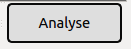
\includegraphics[scale=0.5]{images/bouton_1.png}
	\end{center}
	\caption{L'apparence du bouton "Analyse"}
\end{figure}

La fonction du bouton "Analyse" est celle que nous avions attribué à la touche Entrée. Cette dernière permettait à Yacc de se lancer et d'analyser syntaxiquement le code du fichier courant. Cette fonction était dans le module "editeur" sous le nom de "keyPressEvent" et exécutait différentes actions en fonction de la touche de clavier pressée. J'ai donc juste déplacé le code de la touche Entrée dans une nouvelle fonction nommée "analyse" (toujours dans ce même module).\\

Le problème qui s'est posé fut le suivant : la fenêtre ne s'ouvrait pas, alors que la fonction était bonne et que le bouton lui était relié correctement. Car lors de l'ouverture de l'IDE, aucun QTabWidget n'est ouvert, puisque nous avons fait en sorte qu'il faille ouvrir un projet pour créer un nouveau fichier de code (et donc un nouveau QTabWidget). Nous avons donc réalisé une nouvelle fonction pour le bouton, "pre\_analyse". Celle-ci va tester si il existe au moins un QTabWidget. Si non, alors un message s'affiche disant "Veuillez ouvrir un fichier.". Si oui, alors on appelle la fonction "analyse" et on affiche un message : "Le fichier a bien été analysé.".\\

\begin{figure}
	\begin{center}
		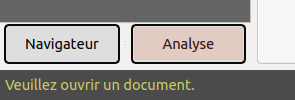
\includegraphics[scale=0.5]{images/bouton_2.png}
	\end{center}
	\caption{"Le message lorsqu'aucun fichier n'est ouvert."}
\end{figure}

\begin{figure}
	\begin{center}
		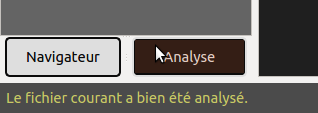
\includegraphics[scale=0.5]{images/bouton_3.png}
	\end{center}
	\caption{"Le message lorsqu'un fichier est ouvert."}
\end{figure}


\end{document}